\documentclass[12pt]{standalone}
\usepackage{tikz}
\usetikzlibrary{arrows.meta}

\usepackage{anyfontsize} % allows arbitrary font sizes
\usepackage{lmodern} % better font scaling

\makeatletter
\renewcommand\normalsize{%
  \@setfontsize\normalsize{16pt}{19pt}%
}
\makeatother

% Tapered stroke: stacked copies, each thicker and started further along,
% so the line grows from a thin tail into the head.  #1 = style, #2 = path.
\newcommand{\taperline}[2][]{%
  \foreach \i in {1,...,10}{%
    \pgfmathsetmacro{\tw}{2.2*\i/10}%
    \pgfmathsetmacro{\ts}{1.2*(\i-1)}%
    \draw[#1, line width=\tw pt, shorten <=\ts pt,
          line cap=round, line join=round, rounded corners=4pt] #2;%
  }%
}
\newcommand{\taperarrow}[2][]{%
  \taperline[#1]{#2}%
  \draw[#1, line width=2.2pt, shorten <=12pt, rounded corners=4pt,
        -{Stealth[length=8pt,width=7pt]}] #2;%
}

\begin{document}

\begin{tikzpicture}[
  thick, scale=1.2,
  small label/.style={
    anchor=north west, font=\scriptsize, xshift=-3pt, yshift=3pt, blue, overlay
  },
  flow/.style={red!75!black, line cap=round, line join=round},
  acc/.style={red!75!black, inner sep=1pt}
]
\draw[fill=red!15, draw=none, overlay] (4.35,0.1) rectangle (8.75,-6.6);
\draw (0,0) node[small label] {1} rectangle (10.9,-1.15);
\node at (5.45,-0.315) {$s=42$};
\node[red!75!black] at (5.45,-0.835) {$t=1$};
\draw (0,-1.8) node[small label] {2} rectangle (6.5,-2.95);
\node at (3.25,-2.115) {$s=22$};
\node[red!75!black] at (3.25,-2.635) {$t=3$};
\draw (0,-3.6) node[small label] {3} rectangle (4.3,-4.75);
\node at (2.15,-3.915) {$s=5$};
\node at (2.15,-4.435) {$t=0$};
\draw (0,-5.4) node[small label] {4} rectangle (2.1,-6.55);
\node at (1.05,-5.715) {$s=4$};
\node at (1.05,-6.235) {$t=0$};
\draw (2.2,-5.4) node[small label] {5} rectangle (4.3,-6.55);
\node at (3.25,-5.715) {$s=1$};
\node at (3.25,-6.235) {$t=0$};
\draw[ultra thick] (4.4,-3.6) node[small label] {6} rectangle (6.5,-4.75);
\node[red!75!black] at (5.45,-3.915) {$s=8$};
\node at (5.45,-4.435) {$t=5$};
\draw (6.6,-1.8) node[small label] {7} rectangle (10.9,-2.95);
\node at (8.75,-2.115) {$s=15$};
\node[red!75!black] at (8.75,-2.635) {$t=2$};
\draw[ultra thick] (6.6,-3.6) node[small label] {8} rectangle (8.7,-4.75);
\node[red!75!black] at (7.65,-3.915) {$s=6$};
\node at (7.65,-4.435) {$t=4$};
\draw (8.8,-3.6) node[small label] {9} rectangle (10.9,-4.75);
\node at (9.85,-3.915) {$s=5$};
\node at (9.85,-4.435) {$t=0$};
% Each step of the query is its own arrow.
\taperarrow[flow]{(6.2,-4.30) -- (6.2,-3.52)}
\taperarrow[flow]{(7.05,-4.30) -- (7.05,-3.52)}
\taperarrow[flow]{(6.2,-3.03) -- (6.2,-1.72)}
\taperarrow[flow]{(7.05,-3.03) -- (7.05,-1.72)}
\taperarrow[flow]{(6.20,-1.23) -- (6.55,-0.90)}
\taperarrow[flow]{(7.05,-1.23) -- (6.71,-0.90)}
\taperarrow[flow]{(6.63,-0.88) -- (6.63,-0.26)}
\node[acc] at (6.20,-3.275) {$8$};
\node[acc] at (7.05,-3.275) {$6$};
\node[acc,font=\footnotesize] at (5.60,-2.375) {$+\,3\times 1$};
\node[acc,font=\footnotesize] at (7.62,-2.375) {$+\,2\times 1$};
\node[acc] at (6.20,-1.475) {$11$};
\node[acc] at (7.05,-1.475) {$8$};
\node[acc,font=\footnotesize] at (7.25,-0.625) {$+\,1\times 2$};
\node[acc] at (6.63,0.35) {$\varphi([3,4])=21$};
\end{tikzpicture}

\end{document}
